\begin{apendicesenv}

\chapter{Exemplo de Apêndice}
\label{cap:apendice}

    Exemplo de Apêndice. Aqui, aproveitamos para descrever a regra para inserção de Figuras. As Figuras devem ser centralizadas, com legenda e fonte descritas alinhadas à esquerda, como pode ser observado pela Figura \ref{fig:exemplo}. O mesmo ocorre para os gráficos, como apresentado pelo Gráfico \ref{fig:exgrafico}.

    \begin{figure}[h]
        \caption{Exemplo de Imagem.}
        \begin{center}
            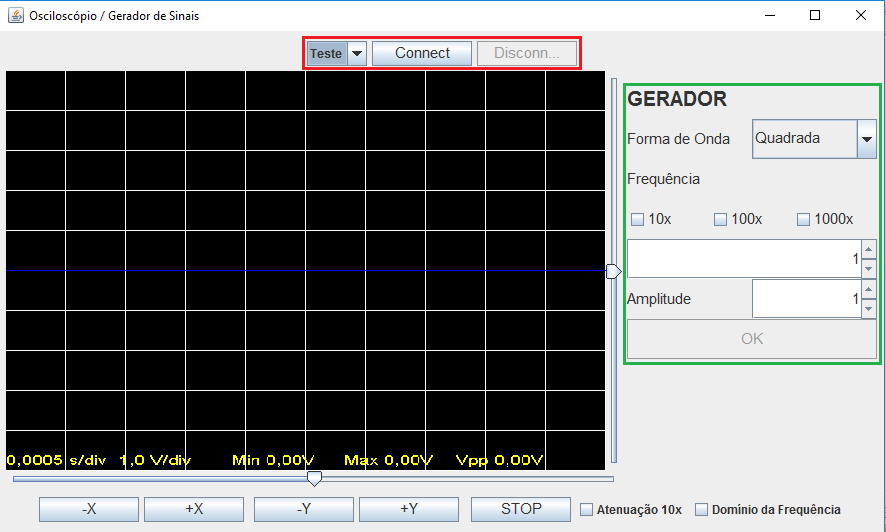
\includegraphics[width=0.6\linewidth]{Imagens/Tela.png}
        \end{center}
        \legend{\small{Fonte: \citeonline{SantanadaSilva2020}}}
        \label{fig:exemplo}
    \end{figure}

    \begin{grafico}[h]
        \caption{Exemplo de Gráfico.}
        \begin{center}
            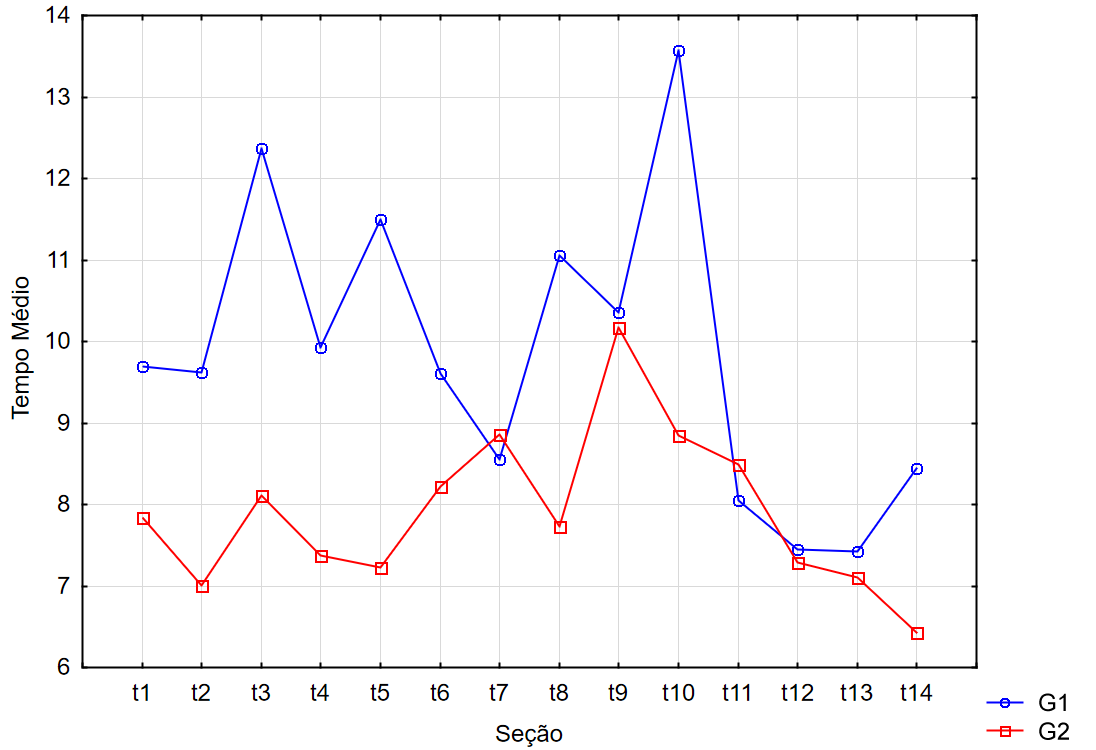
\includegraphics[width=0.6\linewidth]{Imagens/grafico.png}
        \end{center}
        \label{fig:exgrafico}
    \end{grafico}

    Ainda, tabelas que possuem apenas informações textuais, devem ser nomeadas por quadros, como apresenta o Quadro \ref{qua:exemplo}.

    \begin{quadro}[ht]
        \caption{Exemplo de Quadro}
        \begin{tabular}{ll}
            \toprule
            Termo & Significado \\
            \midrule
            char  & Um caractere, ou valor inteiro não sinalizado com 8 bits \\
            int   & Valor numérico com 4 bytes de comprimento \\
            \bottomrule
            \bottomrule
        \end{tabular}
        \label{qua:exemplo}
    \end{quadro}

\end{apendicesenv}
